\scanpage{76}
En effet, \deleted{\unsure{quitte}} on peut supposer \inserted{$S,T$ connexes réduits, donc $T$ un tore} \deleted{\unsure{déployés : par une extension} \inserted{finie} de $k$, \unsure{que} $T$ et le tore \unsure{maximal} $S_0$ de $S$}.
On peut supposer aussi $S$ extension d'une VA par un tore $S_0$. Quitte à faire une extension finie, on peut supposer
\[
S_0\simeq\mathbf G_m^r,\qquad T\simeq\mathbf G_m^s.
\]
Alors $T_\ell(S_0)\times T_\ell(T)\mathbin{-}T_\ell(\mathbf G_m)$ est un accouplement
\[
\mathbf Z_\ell^r\otimes\mathbf Z_\ell^s\mathbin{-}\mathbf Z_\ell^{\unsure{s|1}},
\]
où \deleted{$\unsure{\mathbf Z_\ell}$} l'élém. $f$ de Frob. opère sur \deleted{$\mathbf Z_\ell$} les trois facteurs par $q\,\mathrm{id},q\,\mathrm{id},q\,\mathrm{id}$, donc sur le premier \unsure{mb.} par $q^2\,\mathrm{id}$, sur le dernier par $q\,\mathrm{id}$. Donc l'accouplement induit est nul. Cela nous ramène au cas où $S$ est une V.A. Mais par Weil, les val. propres de $f$ opérant sur $\deleted{\unsure{\mathbf Z_\ell}}T_\ell(S)$ sont de val. absolue $q^{1/2}$, donc les val. propres sur $T_\ell(S)\otimes T_\ell(\mathbf G_m)$ sont de val. absolue $q^{3/2}$, et sur $T_\ell(\mathbf G_m)$ on a $q$, on a encore nullité.
\figure{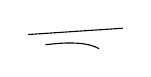
\begin{tikzpicture}\draw (0,0)--(1.2,.08);\draw (.22,-.13)..controls (.6,-.08) and (.8,-.12)..(.9,-.18);\end{tikzpicture}}

Nous traitons maintenant le cas général, \deleted{Pour cela}, \unsure{qui, nous le savons}, se ramène au cas $X$ un trait \inserted{$=\operatorname{Spec}V$, \unsure{de val. discr.}} $Y$ son pt fermé. On écrit
\[
V=\varinjlim A_i,\qquad A_i\subset V,\qquad A_i\deleted{\unsure{étant}}\text{ de t.f. sur }\mathbf Z.
\]
\deleted{\unsure{Pour ce faire}} Soit
\[
X_i=\operatorname{Spec}A_i,\quad Y_i=V(\unsure{\mathfrak p_i|p_i}),\quad U_i=X_i-Y_i;
\]
donc
\[
X=\varprojlim X_i,\quad Y=\varprojlim Y_i,\quad U=\varprojlim U_i.
\]
\margin{75}
